% ----------------------------------------------------------
\chapter{Estado da Arte}
% ----------------------------------------------------------

\section{Métodos de Escavação}

Há diversas formas de se executar túneis, tanto profundos quanto superficiais. Durante a escolha do método de escavação, o engenheiro deve levar em conta diversos fatores, tais como: geometria da seção, comprimento do túnel, condições geológicas, nível da água, restrições quanto às vibrações, estabilidade da cavidade, riscos de assentamentos superficiais, hipóteses de projeto, segurança dos operários, viabilidade ambiental e econômica. Em vista dessa complexidade é possível utilizar mais de um método de escavação ao longo do eixo do túnel. A \autoref{metodos_escavacao} resume os principais métodos de escavação.

\begin{figure}[H]
	\begin{center}
		\includegraphics[scale = 1]{0301-métodos de escavação de túneis.pdf}
	\end{center}
	\caption{\label{metodos_escavacao}Métodos de escavação de túneis}
\end{figure}

Os métodos se dividem em dois grandes grupos: 1) não mecanizados (convencionais) e 2) mecanizados. A diferença é que este último é caracterizado pela presença de tuneladoras, que são máquinas especializadas em adentrar a frente de escavação. Os métodos ditos “não mecanizados”, não possuem essas máquinas especializadas, e podem ser agrupados em: vala recoberta, escavação simples e desmonte de rocha.

\subsection{Vala recoberta}

O método da vala recoberta é utilizado preferencialmente para túneis superficiais (conhecido também, nas cidades, como método a céu aberto). Pode ser executado de duas formas: direta (\textit{Cut and Cover}) ou invertida (\textit{Cover and Cut}). A \autoref{vala_recoberta} e \autoref{etapa_execucao_vala_recoberta} ilustram esse método.

\begin{figure}[H]
	\begin{center}
		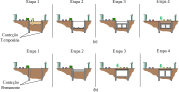
\includegraphics[scale = 0.8]{0302-vala recoberta.pdf}
	\end{center}
	\caption{\label{vala_recoberta}(a) \textit{Cut and Cover} e (b) \textit{Cover and Cut} (adaptado de: \citeonline[p. 5-2]{FederalHighwayAdministration2009})}
\end{figure}

\begin{figure}[H]
	\begin{center}
		\includegraphics[scale = 1]{0303-etapa de execução pelo método de vala recoberta direta.jpg}
	\end{center}
	\caption{\label{etapa_execucao_vala_recoberta}Etapa de execução pelo método de vala recoberta direta no projeto \textit{Nordhavnsvej}, em Compenhague, Dinamarca (fonte: \citeonline[p. 1]{ROADTRAFFIC-TECHNOLOGY2019})}
\end{figure}

Como o presente trabalho está delimitado aos túneis profundos esse método de escavação estará fora do escopo desta tese. Além disso, o comportamento mecânico desse tipo de túnel é diverso dos profundos que, tal como será visto no Capítulo 4, mobilizam a resistência do maciço na estabilidade da cavidade.


\subsection{Escavação simples}

A escavação simples é o método que permite maior flexibilidade quanto à geometria da seção e é ideal para escavar galerias de formatos complexos, como por exemplo, estações e conexões. Essa escavação pode ser feita com uma combinação de ferramentas que vão desde manuais até equipamentos mecânicos, como escavadeira simples, escavadeira rotativa (\textit{Roadheader}), escarificador e martelo hidráulico (\textit{Hammerhead}) (\autoref{escavadeiras}). A produtividade desse método varia, mas dificilmente ultrapassa 10m/dia de avanço.

\begin{figure}[H]
	\begin{center}
		\includegraphics[scale = 1]{0304-escavadeiras,escarificadora,rotativa e martelo hidraulico.jpg}
	\end{center}
	\caption{\label{escavadeiras}Superior à esquerda: escavadeiras (fonte: \citeonline[p. 1]{Pierrat2014}); superior à direita: escarificadora; inferior à esquerda: escavadeira rotativa (fonte: \citeonline[p. 1]{Mitterndorfer2013}) e inferior à direita: martelo hidráulico  (fonte: \citeonline[p. 1]{WORDHIGHWAYS2015})}
\end{figure}


\subsection{Desmonte de rocha}

Quando há dificuldade de penetração no maciço, é necessário utilizar o método de perfuração e detonação, que consiste em perfurar, instalar o material explosivo e detonar a frente de escavação. O ciclo desse tipo de escavação é ilustrado na \autoref{sequencia_detonacao} e \autoref{sequencia_detonacao_fotos}.

\begin{figure}[H]
	\begin{center}
		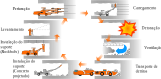
\includegraphics[scale = 1]{0305-sequencia detonação.pdf}
	\end{center}
	\caption{\label{sequencia_detonacao}Sequência executiva do método de construção por desmonte de rocha (adaptado de: \citeonline[p. 215]{Heinio1999})}
\end{figure}

\begin{figure}[H]
	\begin{center}
		\includegraphics[scale = 0.6]{0306-perfuracao,instalacao das cargas e frente detonada.png}
	\end{center}
	\caption{\label{sequencia_detonacao_fotos}Superior à esquerda: perfuração; inferior à esquerda: instalação das cargas; à direita: frente de escavação após detonação (fonte: \citeonline[p. 1]{Grad2013})}
\end{figure}

\subsection{Tuneladora}

As tuneladoras, tal como ilustrada na \autoref{representacao_tuneladora}, nada mais são do que a evolução do método de escavação com plataformas de Marc Brunel desenvolvido em 1843 (durante a construção do túnel subfluvial sob o Tâmisa em Londres). Hoje em dia, essa escavação é totalmente mecanizada e possui excelente regularidade da superfície escavada. A produtividade depende de vários fatores (diâmetro da seção do túnel, condições do maciço, potência e tamanho da máquina, projeto de suporte, experiência das equipes) e pode atingir até 20m/dia \cite[p. 98]{Brox2017}. Geralmente possuem maquinário acoplado para executar o revestimento em concreto projetado ou anéis de concreto pré-moldados. Quando o maciço a ser escavado é pouco resistente é utilizado um escudo (\textit{Shield}) ou lama sob pressão imediatamente anterior à frente de escavação para evitar o colapso da cavidade. As principais desvantagens são o custo e a dificuldade de transporte da máquina.

\begin{figure}[H]
	\begin{center}
		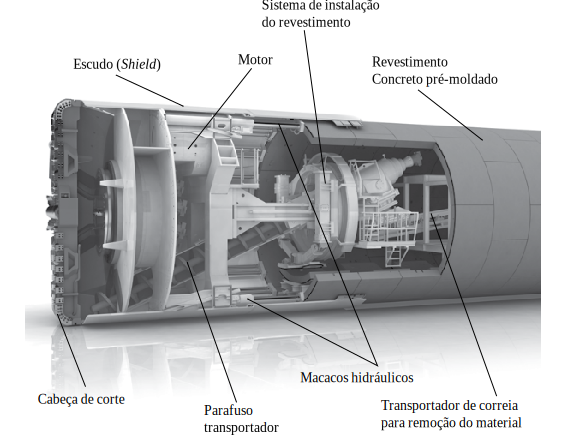
\includegraphics[scale = 1]{0307-representacao 3D de uma tuneladora.pdf}
	\end{center}
	\caption{\label{representacao_tuneladora}Representação 3D de uma tuneladora (adaptado de: \citeonline[p. 151]{Chapman2018})}
\end{figure}

\subsection{Cravação de tubos}

Por fim, o método mecanizado de cravação de tubos consiste em conectar dois poços cravando tubos com auxílio de macacos hidráulicos, uma parede de reação e uma pequena tuneladora (com ou sem escudo). Esse método é comum quando se tem poucas distâncias a vencer, túneis superficiais e solos brandos. São, portanto, preferencialmente utilizados em obras de fornecimento de água, esgoto, eletricidade e gás nos centros urbanos. A \autoref{cravacao_tubos} e \autoref{cravacao_tubos_fotos} ilustram esse método de escavação.

\begin{figure}[H]
	\begin{center}
		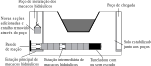
\includegraphics[scale = 1]{0308-metodo de cravacao de tubos.pdf}
	\end{center}
	\caption{\label{cravacao_tubos}Ilustração do método de cravação de tubos sob um canal (adaptado de: \citeonline[p. 227]{Chapman2018})}
\end{figure}

\begin{figure}[H]
	\begin{center}
		\includegraphics[scale = 0.6]{0309-poco de macacos hidraulicos com a descida da TBM.png}
	\end{center}
	\caption{\label{cravacao_tubos_fotos}À esquerda: vista de cima de um poço de macacos hidráulicos com a descida da TBM; à direita: vista frontal do túnel (fonte: \citeonline[p. 227]{Chapman2018})}
\end{figure}

Como este trabalho está delimitado aos túneis profundos, esse método de escavação estará fora do escopo dessa tese. Apesar de mobilizar a resistência do maciço possuí condições de contorno bem diversas de túneis profundos.

\section{Pré-suportes}



\section{Revestimento de túneis}



\section{Principais aspectos considerados em estudos numéricos recentes de túneis}




